% In this file you should put the actual content of the blueprint.
% It will be used both by the web and the print version.
% It should *not* include the \begin{document}
%
% If you want to split the blueprint content into several files then
% the current file can be a simple sequence of \input. Otherwise It
% can start with a \section or \chapter for instance.

\chapter{Notation}\label{subsec:notation}
We aim to make this exposition intuitive for those not specialized in type theory. Hence, we will present the formal specification of the concepts in such a way that they are on the one hand as suggestive for their Lean implementation as possible while at the same time being stated in set theoretic terms rather than type theoretic ones. This made possible by an intuitive correspondence between types and sets (see e.g. \cite{nederpelt:1994}).

Moreover, as Lean has additional functionalities on top of its type theoretic basis to allow for efficient programming and proof verification, some limitations arise preventing the code from following exactly the common conceptualizations of set theoretic mathematics. The most notable of these deviations is that the symbol \texttt{0} in Lean has a reserved meaning, namely \texttt{Nat.zero}, an inhabitant of the primitive type \texttt{Nat}, describing the natural numbers. As we shall also define a language involving the concept of zero, we will hence name it \texttt{null}.

To allow for efficient automatic formulas manipulation, variables bound by a quantifier are associated with De Bruijn \cite{bruijn:1972} indices in \texttt{mathlib}'s implementation of first-order formulas. These indices are natural numbers that correspond to the level-distance between the variable and the quantifier that binds it. Take as an example the regular first-order formula 
\begin{align}
    \forall x (\forall y (P(y) \to R(f(x))) \to (R(z) \to P(a))),
\end{align} where $x, y$ are bound variables, $z$ is a free variables, $P$ and $R$ are predicates and $a$ is a constant.
In De Bruijn notation this formula is expressed by
\begin{align}\label{fml:db}
    \forall (\forall (P(0) \to R(f(1))) \to (R(1) \to P(a))).
\end{align}
Troughout this documentation we will use this formula as illustration to the concepts introduced.

\chapter{Preliminaries}
\section{Syntax}
The ordinary definition of a first-order language $\mathcal{L}$ proceeds from the specification of a signature $\mathcal{S}$ and then an inductive definition of the way formulas can be build with elements from $\mathcal{S}$, the set of logical connectives, variables and the quantifiers. See that for any first order language all these elements except the signature are the same. Hence, we could think of a specific first order language as being fully specified by its signature.

% \begin{definition}[formal language] \label{def:formal-language}
%     Let $\Sigma$ be a set of symbols. Then a formal language $\mathcal{L}$ is a subset of $\Sigma^*$.
% \end{definition}

% \begin{definition}[first-order logical vocabulary]\label{def:FO-logical-vocab}
%     The \textit{first-order logical vocabulary}, is a structure $\mathcal{S} = (\mathcal{V},\neg,\mathcal{B},=,\mathcal{Q},\mathcal{P}, \top, \bot)$ where
%     \begin{enumerate}
%         \item $\mathcal{V} = \{x,y,z,...\}$ is the \textit{set of variables},
%         \item $\neg$ is the \textit{negation operator},
%         \item $\mathcal{B} = \{\land,\lor,\to,\leftrightarrow\}$ is the \textit{set of binary sentential operators},
%         \item $=$ is the \textit{identity predicate},
%         \item $\mathcal{Q} = \{\forall, \exists\}$ is the \textit{set of quantifiers},
%         \item $\mathcal{P} = \{(,)\}$ is the \textit{set of parentheses},
%         \item $\top$ is called \textit{top} and
%         \item $\bot$ is called \textit{bottom}.
%     \end{enumerate}
% \end{definition}

% \begin{definition}[variables]\label{def:FO-variables}
%     We define the set of variables for a first order language as the finite set $\mathcal{V} = \{x,y,z,...\}$.
% \end{definition}

\begin{definition}[first-order language]\label{def:fol}
    \lean{FirstOrder.Language}
    \leanok
    Let $A$ be a set of function symbols and $B$ a set of predicate symbols. Then, a first-order language is a structure $\langle F, R \rangle$, where 
        \begin{enumerate}
            \item $F : \mathbb{N} \to A$ and
            \item $R : \mathbb{N} \to B$.
        \end{enumerate}

    % A language is a structure $((F_i)_{i\in \mathbb{N}}, (R_i)_{i\in \mathbb{N}})$, where $F_i$ is a set of $i$-ary function symbols and $R_i$ a set of $i$-ary predicate symbols.
\end{definition}

Note that this defines a language as consisting only of functions and relations, whereas traditionally a language also contains a set of constants. Observe, however, that constants can be modelled as $0$-ary functions, so this definition of a language does not limit expressive power. By providing concrete sets of function and relation symbols to $F_i$ and $R_i$ we obtain a specific language. 

We will be implementing the languages $\mathcal{L}$ and $\mathcal{L}_T$ that are necessary for the proof of Halbach's \cite{halbach2011} Theorem 7.5 of the conservativity of \texttt{TB} and \texttt{UTB} over \texttt{PA}.

\begin{definition}[$\mathcal{L}$: the language of peano arithmetic with syntactic functions and predicates]\label{def:l}
    \uses{def:fol}
    \lean{Languages.L.signature}
    \leanok
    The language of peano arithmetic including syntactic functions and predicates is the first-order language $\mathcal{L} = \langle F, R \rangle$, where
    \begin{enumerate}
        \item $F$ is defined by
        \begin{enumerate}
            \item $F(0) = \{\texttt{null}\}$,
            \item $F(1) = \{\texttt{succ},\texttt{num}¸\texttt{neg},\texttt{forall},\texttt{exists},\texttt{denote}\}$,
            \item $F(2) = \{\texttt{add},\texttt{mult},\texttt{conj},\texttt{disj},\texttt{cond}\}$ and
            \item $F(3) = \{\texttt{subs}\}$ and 
        \end{enumerate}
        \item $R$ is defined by \item $R(1) = \{\texttt{Variable},\texttt{Constant},\texttt{ClosedTerm},\texttt{Term},\texttt{Formula}_{\mathcal{L}}, \texttt{Sentence}_{\mathcal{L}},\texttt{Formula}_{\mathcal{L}_T},\texttt{Sentence}_{\mathcal{L}_T}\}.$
    \end{enumerate}
\end{definition} 

\begin{definition}[$\mathcal{L}_{T}$: the language of peano arithmetic including the truth predicate symbol]\label{def:lt}
    \uses{def:fol, def:l}
    \lean{Languages.L_T.signature}
    \leanok
    Let $\mathcal{L} = \langle F_{\mathcal{L}},R_{\mathcal{L}} \rangle$ be the language of peano arithmetic including syntactic functions symbols and predicates. Then, the language $\mathcal{L}_T$ is the first-order language $\mathcal{L}_T = \langle F, R \rangle$, where
    \begin{enumerate}
        \item $F = F_{\mathcal{L}}$ and
        \item $R$ is defined by $R(1) = R_{\mathcal{L}}(1) \cup \{\texttt{Tr}\}$.
    \end{enumerate}
\end{definition}

We can then work our way up, first to the level of terms and then that of formulas. For this, we use \texttt{mathlib}'s implementation of \texttt{Term}s and \texttt{BoundedFormula}s. 

% As \cite{ffl} want to be able to make a distinction between sentences, i.e. formulas without free variables, and non-sentences, i.e. formulas containing free variables, their formalization of formulas features a distinction between bound and free variables, something which is not present in traditional de Bruijn syntax, where free variables are just those that are indexed by a number higher than the amount of quantifiers ($-1$ as Lean 4 is 0-based). For example in the de-Bruijn style formula 
% \begin{equation}
% \forall P(0,1),
% \label{eq:db}
% \end{equation}
% the variable indexed by 1 is a free variable, while the variable indexed by 0 is bound by the universal quantifier. In \cite{ffl}'s notation, however, this formula would be coded as
% \begin{equation}
% \forall P(\#0,\&0),
% \label{eq:ffl}
% \end{equation}
% where \& indicates the index following it indexes a free variables and \# indicates the index following it indexes a bound variable. Hence the universal quantifier binds \#0 and not \&0, corresponding to the meaning of expression \ref{eq:db}.

% Another consequence of this distinction is that we need an effective method to ensure all variables that were intended as bound variables are indeed bound by some quantifier. To ensure that is the case \cite{ffl}'s authors make use of \textit{partially applied} formulas, called semi-formulas, that have a parameter $n \in \mathbb{N}$ measuring the difference between the intended and present number of quantifiers. As a result, $n$ also indicates the number of distinct bound variables the semi-formula may contain that do not yet have a corresponding quantifier. The idea is that these $n$ quantifiers will still be added. 

% Pried loose from the ordered nature of indexing that only bound variable match-up with quantifiers requires it is now also possible, for abstraction purposes, to have the free variables indexed by an aribitrary set rather than an ordered one. Nevertheless, for most purposes using $\mathbb{N}$ for free variable indexing is convenient.


% % Now, assuming expression \ref{eq:ffl} is a well-formed formula, we should, by the above concept of \textit{partially applied formulas}, have that its sub-formula $\varphi = P(\#0,\&0)$ has a parameter $n = 1$ specifying one quantifier should be added to $\varphi$ to obtain a well-formed formula. As will become apparent from Definition \ref{def:sem-t} and Definition \ref{def:sem-f}.3 this is exactly why $P(\#0,\&0)$ can contain \#0 as a term in the first place: Definition \ref{def:sem-f}.3 and Definition \ref{def:sem-f}.4 state that semiformulas of the set with $n = k$ can only contains semiterms from the set of semiterms with $n = k$ and sets of semi-terms with parameter $n$ can only contain bound variables $\#i$ with $i < n$. Together with Definitions \ref{def:sem-f}.7 and \ref{def:sem-f}.8 this assures that in formulas in the set of semiformulas with $n = 0$ all bound variables are bound.
% %  then assure that whenever a quantifier $Q$ is placed in front of a formula $\psi$ from the set of semiformulas with parameter $n = k$ the resulting formula $Q \psi$ is a member of the set of semiformulas with parameter $n = k - 1$. So the only way to obtain a semiformula in the set with $n = k - 1$ is to either (i) place a quantifier in front of a semiformula from the set with $n = k$, all of which only require $k$ extra quantifiers before the formula is well-formed or (ii) construct a semiformula that only contains bound variables that require $k - 1$ quantifiers before the formula to make it well-formed. Hence, a semiformula from the set with $n = 0$ can be obtained by either (i) placing a quantifier in front of a semiformula from the set of semiformulas that only need $n = 1$ extra quantifier to make them well-formed or (ii) by constructing a semiformula that only contains bound variables that require $0 - 1 \in \mathbb{N}$, i.e. no, quantifiers to make it well-formed. This guarantees that all formulas in the set of semiformulas with $n = 0$ are well-formed.

\begin{definition}[Term]\label{def:term}
    \uses{def:fol}
    \lean{FirstOrder.Language.Term}
    \leanok
    Let $\mathcal{L} = \langle F, R \rangle$ be a first-order language and $\alpha$ a set used to index free variables. Then the set of terms with respect to $\mathcal{L}$ and $\alpha$ denoted $\mathcal{T}(\mathcal{L},\alpha)$ is the smallest set such that
        \begin{enumerate}
            \item the set of variables with respect to $\alpha$ denoted $\mathcal{V}(\alpha) = \{x_i | i \in \alpha\} \subseteq \mathcal{T}(\mathcal{L},\alpha)$ and
            \item for all $i \in \mathbb{N}$, if $f \in F(i)$ and $x_1,...,x_i \in \mathcal{T}(\mathcal{L},\alpha)$, then $f(x_1,...,x_i) \in \mathcal{T}(\mathcal{L},\alpha)$.
        \end{enumerate}
\end{definition}

% \begin{definition}[semi-term]\label{def:sem-t}
%     \uses{def:fol}
%     \lean{LO.FirstOrder.Semiterm}
%     \leanok
%     Let $\mathcal{L} = \langle F, R \rangle$ be a first-order language, $\xi$ a set used for indexing of free variables and $n \in \mathbb{N}$ an intended number of quantifiers. Then, the set of semi-terms $A_{\mathcal{L},\xi,n}$ is the smallest set such that
%     \begin{enumerate}
%         \item the set of bound variables $BV_n = \{\#i | 0 \leq i < n\} \subseteq A_{\mathcal{L},\xi,n}$,
%         \item the set of free variables $FV_\xi = \{\&i | i \in \xi\} \subseteq A_{\mathcal{L},\xi,n}$ and
%         \item for all $i \in \mathbb{N}$, if $f \in F(i)$ and $x_1,...,x_i \in A_{\mathcal{L},\xi,n}$, then $f(x_1,...,x_i) \in A_{\mathcal{L},\xi,n}$.
%     \end{enumerate}
% \end{definition}

% Subsequently, we define full syntactic terms from this by setting $\xi = \mathbb{N}$, as we are using de Bruijn indexing to index our free variables, and $n = 0$, as syntactic terms are not bound variables.

% \begin{definition}[syntactic term]\label{def:syn-t}
%     \uses{def:fol, def:sem-t}
%     \lean{LO.FirstOrder.SyntacticTerm}
%     \leanok
%     Let $\mathcal{L}$ be a first-order language. Then, the set of syntactic terms $\mathcal{T}_{\mathcal{L}}$ associated with this language is the set of semi-terms $A_{\mathcal{L},\mathbb{N},0}$. 
% \end{definition}

The concept of \texttt{Term} is used to define the concept \texttt{BoundedFormula}.

\begin{definition}[BoundedFormula]\label{def:bf}
    \uses{def:fol,def:term}
    \lean{FirstOrder.Language.BoundedFormula}
    \leanok
    Let $\mathcal{L} = \langle F, R \rangle$ be a first-order language, $\alpha$ a set indexing free variables, $n$ the intended number of variables bound by a quantifier and $\mathcal{T}(\mathcal{L}, \alpha \cup \{x_1,...,x_n\})$ a set of terms. Then, the set of bounded formulas with respect to these variables $\mathcal{B}(\mathcal{L},\alpha,n)$ is the smallest set such that
    \begin{enumerate}
        \item $\bot \in \mathcal{B}(\mathcal{L},\alpha,n)$,
        \item if $t_1,t_2 \in \mathcal{T}(\mathcal{L}, \alpha \cup \{x_1,...,x_n\})$, then $t_1 = t_2 \in \mathcal{B}(\mathcal{L},\alpha,n)$,
        \item for all $i \in \mathbb{N}$, if $P \in R(i)$ and $t_1,...,t_i \in \mathcal{T}(\mathcal{L}, \alpha \cup \{x_1,...,x_n\})$, then $P(t_1,...,t_i) \in \mathcal{B}(\mathcal{L},\alpha,n)$,
        \item if $f_1,f_2 \in \mathcal{B}(\mathcal{L},\alpha,n)$, then $(f_1 \Rightarrow f_2) \in \mathcal{B}(\mathcal{L},\alpha,n)$ and
        \item if $f \in \mathcal{B}(\mathcal{L},\alpha,n+1)$, then $\forall f \in \mathcal{B}(\mathcal{L},\alpha,n)$.
    \end{enumerate}
\end{definition}

% \begin{definition}[semi-formula]\label{def:sem-f}
%     \uses{def:fol,def:sem-t}
%     \lean{LO.FirstOrder.Semiformula}
%     \leanok
%     Let $\mathcal{L} = \langle F, R \rangle$ be a first-order language, $\xi$ a set used for indexing of free variables, $n \in \mathbb{N}$ an intended number of quantifiers and $A_{\mathcal{L},\xi,n}$ the associated set of semi-terms. Then, the set of semi-formulas $B_{\mathcal{L},\xi,n}$ is the smallest set such that 
%     \begin{enumerate}
%         \item $\texttt{verum} \in B_{\mathcal{L},\xi,n}$,
%         \item $\texttt{falsum} \in B_{\mathcal{L},\xi,n}$,
%         \item for all $i \in \mathbb{N}$, if $P \in R(i)$ and $a_1,...,a_i \in A_{\mathcal{L},\xi,n}$, then $P(a_1,...,a_i) \in B_{\mathcal{L},\xi,n}$,
%         \item for all $i \in \mathbb{N}$, if $P \in R(i)$ and $a_1,...,a_i \in A_{\mathcal{L},\xi,n}$, then $\neg P(a_1,...,a_i) \in B_{\mathcal{L},\xi,n}$,
%         \item if $\varphi_1,\varphi_2 \in B_{\mathcal{L},\xi,n}$, then $\texttt{and}(\varphi_1,\varphi_2) \in B_{\mathcal{L},\xi,n}$,
%         \item if $\varphi_1,\varphi_2 \in B_{\mathcal{L},\xi,n}$, then $\texttt{or}(\varphi_1,\varphi_2) \in B_{\mathcal{L},\xi,n}$,
%         \item if $\varphi_1 \in B_{\mathcal{L},\xi,n+1}$, then $\texttt{all}(\varphi_1) \in B_{\mathcal{L},\xi,n}$ and
%         \item if $\varphi_1 \in B_{\mathcal{L},\xi,n+1}$, then $\texttt{ex}(\varphi_1) \in B_{\mathcal{L},\xi,n}$.
%     \end{enumerate}
% \end{definition}

A \texttt{Formula} is defined as a \texttt{BoundedFormula} that has no variables that still need to be bound.

\begin{definition}[Formula]\label{def:formula}
    \uses{def:fol,def:bf}
    \lean{FirstOrder.Language.Formula}
    \leanok
    Let $\mathcal{L}$ be a first-order language and $\alpha$ a set indexing variables. Then the set of formulas with respect to $\mathcal{L}$ and $\alpha$ denoted $\mathcal{F}(\mathcal{L},\alpha)$ is defined as the set of bounded formulas $\mathcal{B}(\mathcal{L},\alpha,0)$.
\end{definition}

A \texttt{Sentence} is then defined as a \texttt{Formula} that has no free variables.

\begin{definition}[Sentence]\label{def:sentence}
    \uses{def:fol,def:bf}
    \lean{FirstOrder.Language.Formula}
    \leanok
    Let $\mathcal{L}$ be a first-order language. Then the set of sentences with respect to $\mathcal{L}$ denoted $\mathcal{S}(\mathcal{L})$ is defined as the set of formulas $\mathcal{F}(\mathcal{L},\emptyset)$.
\end{definition}

% \begin{definition}[syntactic formula]\label{def:syn-f}
%     \uses{def:fol,def:sem-f}
%     \lean{LO.FirstOrder.SyntacticFormula}
%     \leanok
%     Let $\mathcal{L}$ be a language. Then the set of syntactic formulas $W_{\mathcal{L}}$ associated with this language is the set of semi-formulas $B_{\mathcal{L},\mathbb{N},0}$.
% \end{definition}

% \section{Proof Theory}
% Once we have a formal language and specification of its formulas, we can define a proof system. Proof systems require three elements:
% \begin{enumerate}
%     \item a formal language,
%     \item a set of formulas in the language that function as axioms and
%     \item a set of rules for deriving formulas from other formulas.
% \end{enumerate}    

% We will here define proof systems for $\texttt{PA}$ and $\texttt{PAT}$. To that end we will need these theories' axioms and derivation rules for first-order languages. In \cite{ffl} theories are indexed by their defining axioms, so constructing a theory is equivalent to specifying its defining axioms. 

% \begin{definition}[theory]\label{def:theory}
%     \uses{def:fol,def:syn-f}
%     \lean{LO.FirstOrder.Theory}
%     \leanok
%     Let $\mathcal{L}$ be a formal language and $W_{\mathcal{L}}$ its associated set of syntactic formulas. Then, a theory $T_{\mathcal{L}}$ of $\mathcal{L}$ is a set of syntactic formulas $X$ such that $X \subset W_{\mathcal{L}}$.
% \end{definition}

% Furthermore, we can use \cite{ffl}'s derivation rules that are based on tait calculus (see for example \cite{lee2007}). These rules depend on the concept of substitution of terms in terms and formulas with free bound variables. Traditionally, for example in \cite{negri2001}, substitution is inductively defined over terms, then over formulas. For reasons of integration with Lean 4's preset notions of substitution of terms (Lean 4 is after all a logical system in itself), \cite{ffl} has chosen to not define their substitution methods themselves but rely on Lean 4's innate function for substitution. As the inner workings of Lean 4 are outside the scope of this project and characterizations using the traditional accounts of these operations can be given that function equivalently on the current level of term and formula substitution we will give the traditional definitions of substitution, with the exception that the denotation of term substitution will not resemble that of substitution of terms in formulae, accentuating the fact that $t_0/[t_1]$, where $t_0$ and $t_1$ are semiterms, is not defined in Lean 4.

% \begin{definition}[substitution in terms]\label{def:sub-t}
%     \uses{def:sem-t}
%     \leanok
%     Let $\mathcal{A} = A_{\mathcal{L},\mathbb{N},n}$ and $\mathcal{T} = A_{\mathcal{L},\mathbb{N},n}$ be sets of semiterms. Then, the substitution function $\texttt{sub}_t : \mathcal{A} \times \mathcal{T}^n \to \mathcal{A}$, where $\textbf{t}$ denotes $(t_1,...,t_n)$ is recursively defined as
%     \begin{enumerate}
%         \item if $a = \#i \in BV_n$, then $\texttt{sub}_t(a,\textbf{t}) = t_i$,
%         \item if $a \in FV_{\mathbb{N}}$, then $\texttt{sub}_t(a,\textbf{t}) = a$ and
%         \item if $a = f(b_1,...,b_k) \in \mathcal{A}$, then $\texttt{sub}_t(a,\textbf{t}) = f(\texttt{sub}_t(b_1,\textbf{t}),...,\texttt{sub}_t(b_k,\textbf{t}))$. 
%     \end{enumerate}
% \end{definition}

% With this concept we can then define the concept of substitution in formulas.

% \begin{definition}[substitution]\label{def:subst}
%     \uses{def:sem-t,def:sem-f,def:sub-t}
%     \leanok
%     Let $\mathcal{F} = B_{\mathcal{L},\mathbb{N},n}$ be a set of semiformulae and $\mathcal{T} = A_{\mathcal{L},\mathbb{N},n}$ a set of terms. Then, the substitution function $\texttt{sub}_f : \mathcal{F} \times \mathcal{T}^{n} \to \mathcal{F}$, of terms $\textbf{t} \in \mathcal{T}$, where $\textbf{t} = (t_1,...,t_n)$, in formula $\varphi \in \mathcal{F}$, denoted $\varphi/[\textbf{t}]$, is inductively defined as
%     \begin{enumerate}
%         \item $\texttt{verum}/[\textbf{t}] = \texttt{verum}$;
%         \item $\texttt{falsum}/[\textbf{t}] = \texttt{falsum}$;
%         \item if $P(a_1,...,a_k) \in \mathcal{F}$, then $P(a_1,...,a_k)/[\textbf{t}] = P(\texttt{sub}_t(a_1,\textbf{t}),...,\texttt{sub}(a_k,\textbf{t}))$;
%         \item if $\neg P(a_1,...,a_k) \in \mathcal{F}$, then $ \neg P(a_1,...,a_k)/[\textbf{t}] = \neg P(\texttt{sub}_t(a_1,\textbf{t}),...,\texttt{sub}_t(a_k,\textbf{t}))$;
%         \item if $\texttt{and}(\varphi_1, \varphi_2) \in \mathcal{F}$, then $\texttt{and}(\varphi_1, \varphi_2)/[\textbf{t}] = \texttt{and}(\varphi_1/[\textbf{t}],\varphi/[t])$;
%         \item if $\texttt{or}(\varphi_1, \varphi_2) \in \mathcal{F}$, then $\texttt{or}(\varphi_1, \varphi_2)/[\textbf{t}] = \texttt{or}(\varphi_1/[\textbf{t}],\varphi/[\textbf{t}])$;
%         \item if $\texttt{all}(\varphi) \in \mathcal{F}$, then $\texttt{all}(\varphi)/[\textbf{t}] = \texttt{all}(\varphi/[\textbf{t}])$ and
%         \item if $\texttt{ex}(\varphi)\in \mathcal{F}$, then $\texttt{ex}(\varphi)/[\textbf{t}] = \texttt{ex}(\varphi/[\textbf{t}])$.
%     \end{enumerate}
% \end{definition}

% As our derivation rules are over sequents, below we define the concept of a sequent.

% \begin{definition}[sequent]\label{def:seq}
%     \uses{def:fol,def:syn-f}
%     \lean{LO.FirstOrder.Sequent}
%     \leanok
%     Let $\mathcal{L}$ be some formal language and $W_{\mathcal{L}}$ its associated set of syntactic formulae. Then, a sequent of $\mathcal{L}$ is a tuple $(f_1,...,f_n) \in W_{\mathcal{L}}^n$, where $n \in \mathbb{N}$.
% \end{definition}

% Now we have everything in place to define sequent calculus.

% \begin{definition}[sequent calculus]\label{def:seq-calc}
%     \uses{def:fol,def:sem-t,def:theory,def:syn-t,def:subst,def:seq}
%     \lean{LO.FirstOrder.Derivation}
%     \leanok
%     Let $\mathcal{L} = \langle F,R \rangle$ be some formal language, some $T_{\mathcal{L}}$ an associated theory of this language. Then, the set of sequents derivable from $T_{\mathcal{L}}$ is inductively defined as the smallest set of sequents $X$ such that
%     \begin{enumerate}
%         \item if $(f_1,...,f_n) \in X$ and for some $i \in \mathbb{N}$, $P \in R(i)$ and $a_1,...,a_i \in \mathcal{T}_{\mathcal{L}}$, then \\ $(P(a_1...a_n),\neg P(a_1,...,a_n),f_1,...,f_n) \in X$;
%         \item if $(f_1,...,f_n) \in X$, then $(\top,f_1,...,f_n) \in X$;
%         \item if $(\varphi,\psi,f_1,...,f_n) \in X$, then $(\varphi \lor \psi,f_1,...,f_n) \in X$;
%         \item if $(\varphi,f_1,...,f_n) \in X$ and $(\psi,f_1,...,f_n) \in X$, then $(\varphi \land \psi,f_1,...,f_n) \in X$;
%         \item if $(\varphi,f_1,...,f_n) \in X$, then $(\forall \varphi, f_1,...,f_n) \in X$;
%         \item if $(f_1,...,f_n) \in X$ and there is some $t \in \mathcal{T}$ such that $(\varphi /[t],f_1,...,f_n) \in X$, then $(\exists \varphi, f_1,...,f_n) \in X$;
%         \item for $\Delta = (g_1,...,g_k) \in X$ and $\Gamma = (f_1,...,f_n)$ some sequent, if for all $i: 0 \leq i \leq k$ there is some $j: 0 \leq j \leq n$ such that $g_i = f_j$, then $\Gamma \in X$;
%         \item if $(\varphi,f_1,...,f_n) \in X$ and $(\neg \varphi,f_1,...,f_n) \in X$, then $(f_1,...,f_n) \in X$;
%         \item if $\varphi \in T_{\mathcal{L}}$, then $(\varphi) \in X$. 
%     \end{enumerate}
% \end{definition}

% Intuitively, we can think of all distinct formulas comprising our sequents as disjuncts of one big disjunction thereby making one sequent a big disjunction \cite{lee2007}. The derivation rules ensure that only disjuncts can be derived where truth is preserved.

% \section{Pair encoding}
% Formulas in some first-order langauge $\mathcal{L}$ can be encoded to and decoded from natural numbers. An advantage of this is that we can use a language that has natural numbers as terms, in our case $\mathcal{L}_T$ to formulate metatheoretical statements. In this project we make use of pair encoding.

% Pair encoding of sequences is based on a recursive notion of sequence building, where a pairing function encodes two natural numbers into one natural number, where these natural numbers themselves could again be encodings of two natural numbers, allowing encoding of an arbitrarily large sequence. Hence, we first need the pairing function. This function is native to mathlib.

% \begin{definition}[\texttt{pair}]\label{def:pair}
%     \lean{Nat.pair}
%     \leanok
%     The pairing function $\texttt{pair} : \mathbb{N}^2 \to \mathbb{N}$ is defined as 
%     \begin{align*}
%         \texttt{pair}(a,b) = \begin{cases}
%             b \cdot b + a &\text{if } a < b \\
%             a \cdot a + a + b &\text{else}.        
%         \end{cases}
%     \end{align*}
% \end{definition}

% The encoding this results in is illustrated in Figure \ref{fig:pairing-table}.

% \begin{figure}[h]
%     \centering
%     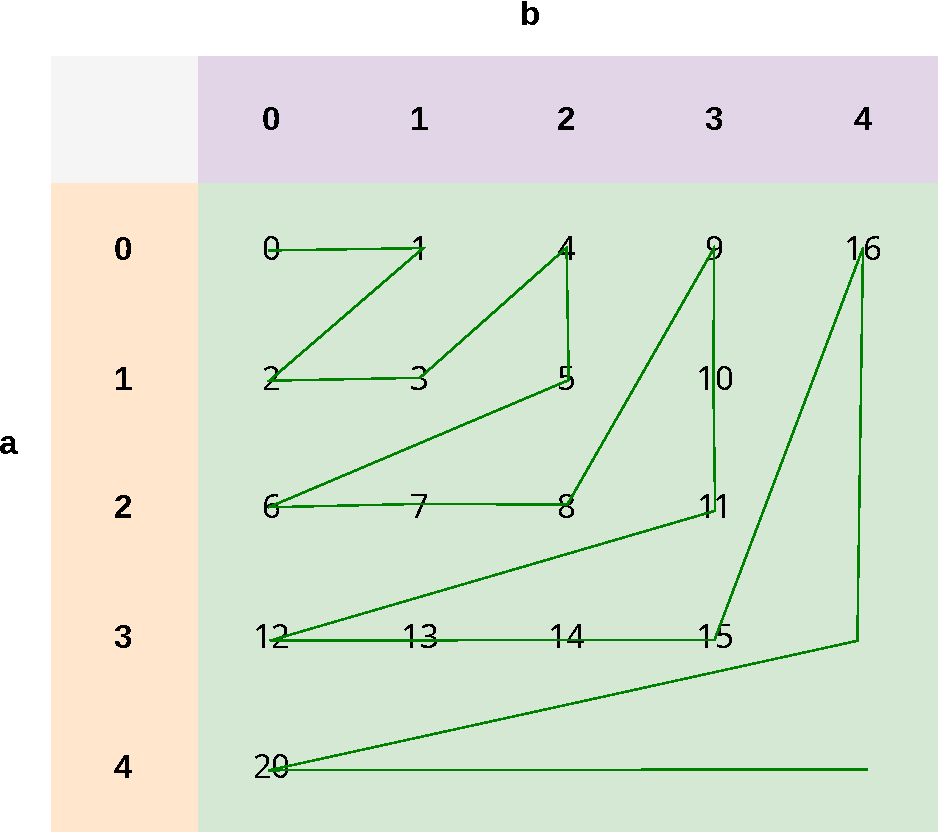
\includegraphics[width=6cm]{./img/pairing-table.pdf}
%     \caption{An illustration of the process of encoding natural numbers using \texttt{pair}.}
%     \label{fig:pairing-table}
% \end{figure}

% Accordingly, we also need a decoding function $\texttt{unpair} : \mathbb{N} \to \mathbb{N}^2$. 

% % \begin{definition}[\texttt{unpair}]\label{def:unpair}
% %     \lean{Nat.unpair}
% %     \leanok
% %     The unparing function \texttt{unpair}$: \mathbb{N} \to \mathbb{N}^2$ is defined as 
% %     \begin{align*}
% %         \texttt{unpair}(n) = \begin{cases}
% %             (0, \sqrt{n}) &\text{if } 0 < \sqrt{n} \\
% %             (\sqrt{n}, - \sqrt{n}) &\text{else}.     
% %         \end{cases}
% %     \end{align*}
% % \end{definition}

% Then, we can use this to have an encoding function $\texttt{toNat} : B_{\mathcal{L},\xi,n} \to \mathbb{N}$ from semiformulas to natural numbers.

% \begin{definition}[\texttt{toNat}]\label{def:toNat}
%     \lean{LO.FirstOrder.Semiformula.toNat}
%     \leanok
%     Let $B_{\mathcal{L},\xi,\mathbb{N}}$ be a set of semiformulas. Then the function $\texttt{toNat} : B_{\mathcal{L},\xi,\mathbb{N}} \to \mathbb{N}$ is defined such that
%     \begin{enumerate}
%         \item \texttt{toNat}$(a,b)$
        
%     \end{enumerate}

% \end{definition}

% \begin{definition}[primitive term]%\label{def:primitive-term}
%     Let $\mathcal{S} = (\mathcal{C},\mathcal{F},\mathcal{R},ar)$ a first-order signature. Then, we define the corresponding set of primitive terms $\mathcal{P}_{\mathcal{S}} = \mathcal{C} \cup \mathcal{V}$.
% \end{definition}

% \begin{definition}[first-order term]%\label{def:FO-term}
%     %\uses{def:FO-logical-vocab, def:FO-signature}
%     Let $\mathcal{S} = (\mathcal{C},\mathcal{F},\mathcal{R},ar)$ be a first-order signature. Then, the set $\mathcal{T}_{\mathcal{S}}$ of \textit{terms} corresponding to $\mathcal{S}$ is recursively defined as the smallest set $X$ such that:
%     \begin{enumerate}
%         \item $\mathcal{P}_{\mathcal{S}} \subseteq X$ and
%         \item if $t_1,...,t_n \in X$, $f \in \mathcal{F}$ and $ar(f) = n$, then $f(t_1,...,t_n) \in X$.
%     \end{enumerate}
% \end{definition}

% \begin{definition}[first-order language]%\label{def:FO-language}
%     %\uses{def:FO-logical-vocab, def:FO-signature, def:FO-term}
%     Let $\mathcal{S} = (\mathcal{C},\mathcal{F},\mathcal{R},ar)$ be a first-order signature. Then the first order language $\mathcal{L}_{\mathcal{S}}$ is recursively defined as the smallest set $X$ such that:
%     \begin{enumerate}
%         \item \begin{enumerate}
%             \item $\top,\bot \in X$,
%             \item if $R \in \mathcal{R}$, $ar(R) = n$ and $t_1,...,t_n \in \mathcal{T}_{\mathcal{S}}$, then $R(t_1,...t_n) \in X$,
%             \item if $t_1,t_2 \in \mathcal{T}_{\mathcal{S}}$, then $t_1 = t_2 \in X$, 
%         \end{enumerate}
%         \item \begin{enumerate}
%             \item if $\phi \in X$, then $\neg \phi \in X$,
%             \item if $\phi, \psi \in X$ then $(\phi \circ \psi) \in X$ for $\circ \in \{\land,\lor,\to,\leftrightarrow\}$ and
%             \item if $x \in \mathcal{V}$ and $\phi \in X$, then $Qx\phi \in X$ for $Q \in \{\forall,\exists\}$.
%         \end{enumerate}
%     \end{enumerate}
% \end{definition}

% \begin{definition}[term's primitive term set]%\label{def:terms-pt-set}
%     Let $\mathcal{S}$ be a first order signature. Then we define the function $tpts_{\mathcal{S}} : \mathcal{T}_{\mathcal{S}} \to \mathcal{P}(\mathcal{P}_{\mathcal{S}})$ mapping terms to the set of primitive terms they contain as
%     \begin{enumerate}
%         \item $tpts_{\mathcal{S}}(s) = \{s\}$ if $s \in \mathcal{P}_{\mathcal{S}}$ and
%         \item $tpts_{\mathcal{S}}(f(t_1,...,t_n)) = tpts_{\mathcal{S}}(t_1)\cup ... \cup tpts_{\mathcal{S}}(t_n)$.
%     \end{enumerate}
% \end{definition}

% \begin{definition}[formula's primitive term set]%\label{FO-term-set}
%     Let $\mathcal{S}$ be a first order signature. We then define the primitive term set function $pts_{\mathcal{S}} : \mathcal{L}_{\mathcal{S}} \to \mathcal{P}_{\mathcal{S}}$ as 
%     \begin{enumerate}
%         \item \begin{enumerate}
%             \item $pts_{\mathcal{S}}(R(t_1,...,t_n)) = tpts_{\mathcal{S}}(t_1) \cup ... \cup tpts_{\mathcal{S}}(t_n)$,
%             \item $pts_{\mathcal{S}}(t_1 = t_2) = tpts_{\mathcal{S}}(t_1) \cup tpts_{\mathcal{S}}(t_2)$,
%         \end{enumerate}
%         \item \begin{enumerate}
%             \item $pts_{\mathcal{S}}(\neg \phi) = pts_{\mathcal{S}}(\phi)$,
%             \item $pts_{\mathcal{S}}((\phi \circ \psi)) = pts_{\mathcal{S}}(\phi) \cup pts_{\mathcal{S}}(\psi)$ for $\circ \in \{\land, \lor, \to, \leftrightarrow\}$,
%             \item $pts_{\mathcal{S}}(Qx\phi) = pts_{\mathcal{S}}(\phi) - \{x\}$ for $Q \in \{\forall, \exists\}$.
%         \end{enumerate}
%     \end{enumerate}
% \end{definition}

% \begin{definition}[substitution function over terms]%\label{def:sub-term}
%     %\uses{def:FO-signature, def:FO-term}
%     Let $\mathcal{S} = (\mathcal{C},\mathcal{F},\mathcal{R},ar)$ be a first order signature. Then, we define the substitution function over terms $subt_{\mathcal{S}} : \mathcal{T}_{\mathcal{S}} \times \mathcal{V} \times \mathcal{T}_{\mathcal{S}} \to \mathcal{T}_{\mathcal{S}}$ recursively such that
%     \begin{enumerate}
%         \item if $s \in \mathcal{P}_{\mathcal{S}}$, then $subt_{\mathcal{S}}(s,x,t) = \begin{cases}
%                         s, &\text{if }s \not = x \\
%                         t, &\text{if }s = x
%                         \end{cases}$
%         \item $subt_{\mathcal{S}}(f(t_1,...,t_n),x,t) = f(subt_{\mathcal{S}}(t_1,x,t),...,subt_{\mathcal{S}}(t_n,x,t))$.
%     \end{enumerate}
% \end{definition}

% % TODO: Proceed here with removing explicit references to the logical vocabulary and indexing the functions on signatures.

% \begin{definition}[substitution function over formulas]%\label{def:sub-f}
%     %\uses{def:FO-signature, def:FO-term, def:FO-language, def:sub-term}
%     Let $\mathcal{S} = (\mathcal{C},\mathcal{F},\mathcal{R},ar)$ a first order signature. Then, we define the substitution function over $\mathcal{L}_{\mathcal{S}}$ as $subf_{\mathcal{S}} : \mathcal{L}_{\mathcal{S}} \times \mathcal{V} \times \mathcal{L}_{\mathcal{S}} \to \mathcal{L}_{\mathcal{S}}$ such that
%     \begin{enumerate}
%         \item \begin{enumerate} 
%             \item $subf_{\mathcal{S}}(R(t_1,...,t_n),x,t) = R(subt_{\mathcal{S}}(t_1,x,t),...,subt_{\mathcal{S}}(t_n,x,t))$,
%             \item $subf_{\mathcal{S}}(t_1 = t_2,x,t) = subt_{\mathcal{S}}(t_1,x,t) = subt_{\mathcal{S}}(t_2,x,t)$
%         \end{enumerate}
%         % TODO : replace sub
%         \item \begin{enumerate}
%             \item $subf_{\mathcal{S}}(\neg \phi,x,t) = \neg subf_{\mathcal{S}}(\phi,x,t)$,
%             \item $subf_{\mathcal{S}}((\phi \circ \psi),x,t) = (subf_{\mathcal{S}}(\phi,x,t) \circ subf_{\mathcal{S}}(\psi,x,t))$, for $\circ \in \{\land,\lor,\to,\leftrightarrow\}$ 
%             \item $subf_{\mathcal{S}}(Qy\phi,x,t)= \begin{cases}
%                 Qy(subf_{\mathcal{S}}(\phi,x,t)) &\text{if } y \not = x \\
%                 Qy\phi &\text{if } y = x
%             \end{cases}$ for $Q \in \{\forall, \exists\}$.
%         \end{enumerate}
%     \end{enumerate}
% \end{definition}

% \begin{definition}[inference rule]%\label{def:inf-rule}
%     %\uses{def:formal-language}
%     Let $\mathcal{L}$ be a formal language. Then an inference rule defined over $\mathcal{L}$ is a function $r : \mathcal{L}^n \to \mathcal{L}$, where $n \in \mathbb{N}$.
% \end{definition}

% \begin{definition}[formal system]%\label{def:formal-system}
%     %\uses{def:formal-language, def:inf-rule}
%     A formal system $\mathcal{S}$ is a structure $\mathcal{S} = (\mathcal{L}, \mathcal{A}, \mathcal{R})$, where 
%     \begin{enumerate}
%         \item $\mathcal{L}$ is a formal language,
%         \item $\mathcal{A} \subseteq \mathcal{L}$ is a \textit{set of axioms} and 
%         \item $\mathcal{R}$ is a \textit{set of inference rules defined over $\mathcal{L}$}.
%     \end{enumerate}
% \end{definition}

% \begin{definition}[sequent set]%\label{def:sequent-set}
%     %\uses{def:formal-language}
%     Let $\mathcal{L}$ be a formal language. Then the set of sequents for that language $\mathcal{S} = \mathcal{P}(\mathcal{L}) \times \mathcal{P}(\mathcal{L})$.
% \end{definition}

% \begin{definition}[sequent calculus inference rules]%\label{def:Rsc}
%     %\uses{def:formal-language, def:sequent-set}
%     Let $\mathcal{L}$ be a formal language and $\mathcal{S}$ the sequent set for $\mathcal{L}$. Then the set of inference rules of sequent calculus is the set $\mathcal{R}_{sc}$ containing the functions
%     \begin{enumerate}
%         \item $r_{ax} : \mathcal{S} \to \mathcal{S}$ defined by $r_{ax}((\emptyset,\emptyset)) = (\{\phi\},\{\phi\})$,
%         \item $r_{cut} : \mathcal{S}^2 \to \mathcal{S}$ defined by $r_{cut}((\Gamma,\Delta \cup \{\phi\}),(\{\phi\} \cup \Sigma,\Pi))=(\Gamma \cup \Sigma, \Delta \cup \Pi)$,
%         \item $r_{\land L_1} : \mathcal{S} \to \mathcal{S}$ defined by $r_{\land L_1}((\Gamma \cup \{\phi\}, \Delta))=(\Gamma \cup \{\phi \land \psi\}, \Delta)$,
%         \item $r_{\land L_2} : \mathcal{S} \to \mathcal{S}$ defined by $r_{\land L_2}((\Gamma \cup \{\psi\}, \Delta))=(\Gamma \cup \{\phi \land \psi\}, \Delta)$,
%         \item $r_{\lor L} : \mathcal{S}^2 \to \mathcal{S}$ defined by $r_{\lor L}((\Gamma \cup \{\phi\},\Delta),(\Gamma \cup \{\psi\},\Delta))=(\Gamma \cup \{\phi \lor \psi\},\Delta)$,
%         \item $r_{\to L} : \mathcal{S}^2 \to \mathcal{S}$ defined by $r_{\to L}((\Gamma, \{\phi\} \cup \Delta),(\Sigma \cup \{\psi\},\Pi))=(\Gamma \cup \Sigma \cup \{(\phi \to \psi)\},\Delta \cup \Pi)$,
%         \item $r_{\neg L} : \mathcal{S} \to \mathcal{S}$ defined by $r_{\neg L}(\Gamma,\{\phi\} \cup \Delta)=(\Gamma \cup \{\neg \phi\},\Delta)$,
%         \item $r_{\forall L} : \mathcal{S} \to \mathcal{S}$ defined by $r_{\forall L}(\Gamma \cup \{\phi [t/x]\},\Delta)=(\Gamma \cup \{ \forall x \phi \},\Delta)$,
%         \item PROCEED HERE
%     \end{enumerate}
% \end{definition}

% \begin{definition}[natural deduction inference rules]%\label{def:Rnd}
%     %\uses{def:FO-language}
%     Let $\mathcal{L}$ be a first order language. Then, the set of inference rules of natural deduction is the set $\mathcal{R}_{nd}$ containing the functions 
%     \begin{enumerate}
%         \item $r_{\land I} : \mathcal{L}^2 \to \mathcal{L}$ defined by $r_{\land I}(\phi,\psi) = \phi \land \psi$,
%         \item $r_{\land E_1} : \mathcal{L} \to \mathcal{L}$ defined by $r_{\land E_1}(\phi \land \psi) = \phi$,
%         \item $r_{\land E_2} : \mathcal{L} \to \mathcal{L}$ defined by $r_{\land E_2}(\phi \land \psi) = \psi$,
%         \item $r_{\lor I_1} : \mathcal{L} \to \mathcal{L}$ defined by $r_{\lor I_1}(\phi) = \phi \lor \psi$,
%         \item $r_{\lor I_2} : \mathcal{L} \to \mathcal{L}$ defined by $r_{\lor I_2}(\psi) = \phi \lor \psi$,
%         \item $r_{\lor E} : \mathcal{L}^3 \to \mathcal{L}$ defined by $r_{\lor E}(\phi \lor \psi, \phi \to \omega, \psi \to \omega)=\omega$,
%         \item $r_{\to E} : \mathcal{L}^2 \to \mathcal{L}$ defined by $r_{\to E}(\phi \to \psi, \phi)=\psi$,
%         \item $r_{\neg I} : \mathcal{L} \to \mathcal{L}$ defined by $r_{\neg I}(\phi \to \bot) = \neg \phi$,
%         \item $r_{\neg E} : \mathcal{L} \to \mathcal{L}$ defined by $r_{\neg E}(\phi, \neg \phi)= \bot$,
%         \item $r_{\bot E} : \mathcal{L} \to \mathcal{L}$ defined by $r_{\bot E}(\bot)=\phi$ and
%         \item $r_{\neg \neg E} : \mathcal{L} \to \mathcal{L}$ defined by $r_{\neg \neg E}(\neg \phi \to \bot)=\phi$,
%         \item PROCEED HERE
%     \end{enumerate}
% \end{definition}

% \begin{definition}[\texttt{PA}: the formal system of Peano arithmetic]%\label{def:PA}
%     %\uses{def:LPA, def:formal-system, def:Rnd}
%     The formal system of Peano arithmetic \texttt{PA} is defined as $\texttt{PA} = (\mathcal{L}_{PA},\mathcal{A},\mathcal{R}_{nd})$, where $\mathcal{A}$ is the smallest set $X$ such that
%     \begin{enumerate}
%         \item $\forall x (0 \not = S(x)) \in \mathcal{A}$, 
%         \item $\forall x,y (S(x) = S(y) \rightarrow x = y) \in \mathcal{A}$,
%         \item $\forall x(x + 0 = x) \in \mathcal{A}$,
%         \item $\forall x,y(x + S(y) = S(x+y)) \in \mathcal{A}$,
%         \item $\forall x(x \cdot 0 = 0) \in \mathcal{A}$,
%         \item $\forall x,y(x \cdot S(y) = x \cdot y + x) \in \mathcal{A}$ and
%         \item if $\varphi(x,y_1,...,y_k) \in \mathcal{L}_{PA}$, then $\bar y \Bigl( \bigl(\varphi(0,\bar y) \land \forall x (\varphi(x,\bar y) \to \varphi(S(x),\bar y))\bigr)\Bigr) \to \forall x \varphi(x, \bar y)$, where $\bar y = y_1,...,y_k$
%     \end{enumerate}
% \end{definition}

% \begin{definition}[formal proof]%\label{def:formal-proof}
%     A formal proof in a logical system $\mathcal{S}$ is a finite sequence of sentences, where each sentence is an axiom of $\mathcal{S}$, an assumption, or follows from the application of one of $\mathcal{S}$'s rules of inference to previous sentences in the sequence (Wikipedia: Formal proof).
% \end{definition}

% \begin{definition}[provability]
%     %\label{def:provable-pa}
%     %\uses{def:formal-proof, def:PA}
%     A formula $\varphi$ is provable in a proof system $\mathcal{S}$ if and only if there exists a formal proof $\mathcal{P}$ in $\mathcal{S}$, such that $\mathcal{P}$ contains no assumptions and $\varphi$ is the last sentence of $\mathcal{P}$.
% \end{definition}

% \begin{definition}[$\mathcal{L}_T$]
%     %\label{def:LT}
%     We define the language $\mathcal{L}_T$ as the language resulting from adding the predicate symbol $T$ to the language $\mathcal{L}$ of \texttt{PA}. 
% \end{definition}

% \begin{definition}[\texttt{PAT}]
%     %\label{def:PAT}
%     %\uses{def:LT}
%     We define the system \texttt{PAT} as the system of Peano arithmetic formulated in $\mathcal{L}_T$ including the induction schema for each formula of the language $\mathcal{L}_T$.
% \end{definition}

\chapter{Axiomatization}\label{chapter:axiomatization}
Once we have a formal language and specification of its formulas, we can define the theories we want to reason about. In \texttt{mathlib} theories are defined by their axioms, so constructing a theory is equivalent to specifying its axioms. 

\begin{definition}[Theory]\label{def:FO-Theory}
  \lean{FirstOrder.Language.Theory}\leanok
  \uses{def:FO-Language,def:FO-Sentence}
  Let $\mathcal{L}$ be a formal language and $S_{\mathcal{L}}$ its associated set of sentences. Then, a theory of $\mathcal{L}$ is a set of sentences $T_{\mathcal{L}}$ such that $T_{\mathcal{L}} \subseteq S_{\mathcal{L}}$.
\end{definition}

We can hence use the notions of $\mathcal{L}$ and $\mathcal{L}_T$ to construct the theories of Syntax Theory, Peano Arithmetic \texttt{PA}, Peano Arithmetic with T \texttt{PAT} and Peano Arithmetic with T and Tarski Biconditionals \texttt{TB}. For Syntax Theory we provide the primitive recursive logical operations as axioms.
\subsubsection{Syntax Axioms}
\begin{definition}[$\underdot{\neg}$: Syntactic Negation Operator Axioms]\label{def:Syntactic-Neg}
  \lean{SyntaxAxioms.neg_repres}\leanok
  \uses{def:FO-Language,def:L,def:FO-Neg,def:L-Numeral}
  The meaning of the syntactic negation operator $\underdot{\neg}$ is captured by the axiom scheme $\mathbb{N})(\underdot{\neg} \ulcorner \varphi \urcorner = \ulcorner \neg \varphi \urcorner)$, where $\varphi \in \mathcal{F}(\mathcal{L},\mathbb{N})$. 
\end{definition}

\begin{definition}[$\underdot{\wedge}$: Syntactic Conjunction Operator Axiom]\label{def:Syntactic-Conj}
  \lean{SyntaxAxioms.conj_repres}\leanok
  \uses{def:FO-Language,def:L,def:FO-And,def:L-Numeral,def:FV-Formula-to-N}
  The meaning of the syntactic conjunction operator $\underdot{\wedge}$ is captured by the axiom scheme $(\ulcorner \varphi \urcorner \underdot{\wedge} \ulcorner \psi \urcorner) = (\ulcorner \varphi \wedge \psi \urcorner)$, where $\varphi, \psi \in \mathcal{F}(\mathcal{L},\mathbb{N})$.
\end{definition}

\begin{definition}[$\underdot{\vee}$: Syntactic Disjunction Operator Axiom Scheme]\label{def:Syntactic-Disj}
  \lean{SyntaxAxioms.disj_repres}\leanok
  \uses{def:FO-Language,def:L,def:FO-Or,def:L-Numeral,def:FV-Formula-to-N}
  The meaning of the syntactic disjunction operator $\underdot{\vee}$ is captured by the axiom scheme $(\ulcorner \varphi \urcorner \underdot{\vee} \ulcorner \psi \urcorner = (\ulcorner \varphi \wedge \psi \urcorner)$, where $\varphi, \psi \in \mathcal{F}(\mathcal{L},\mathbb{N})$.
\end{definition}

\begin{definition}[$\underdot{\supset}$: Syntactic Condition Operator Axiom Scheme]\label{def:Syntactic-Cond}
  \lean{SyntaxAxioms.cond_repres}\leanok
  \uses{def:FO-BoundedFormula,def:L}
  The meaning of the syntactic conditional operator $\underdot{\supset}$ is captured by the axiom scheme $(\ulcorner \varphi \urcorner) \underdot{\supset} \ulcorner \psi \urcorner) = (\ulcorner \phi \supset \psi)$, where $\varphi, \psi \in \mathcal{F}(\mathcal{L},\mathbb{N})$.
\end{definition}

-------------------------------------here should go more syntax axioms-----------------------------------

\begin{definition}[Syntax Theory]\label{def:Syntax-Theory}
  \lean{SyntaxTheory.syntax_theory_l}\leanok
  \uses{def:FO-Theory,def:L}
  We define Syntax Theory as the theory containg all the instances of the axiom schemas for $\underdot{\neg}$, $\underdot{\wedge}$, $\underdot{\vee}$, $\underdot{\supset}$, etc.
\end{definition}

The system of Peano arithmetic contains the defining equations for zero, successor, addition, and multiplication. We first provide the finite theory of the first 6 Peano axioms.
\begin{definition}[The First 6 Axioms of Peano Arithmetic]\label{def:PA-Axioms}
  \lean{PA.peano_axioms}\leanok
  \uses{def:FO-Language,def:FO-Theory,def:L}
    The theory of the first 6 axioms of Peano Arithmetic \texttt{PA-axioms} is defined as the smallest theory $X$ such that
    \begin{enumerate}
        \item $\forall \neg (\&0 = S(\&0) \in X$, 
        \item $\forall \forall (S(\&1) = S(\&0) \rightarrow \&1 = \&0) \in X$,
        \item $\forall (\&0 + \texttt{null} = \&0) \in X$,
        \item $\forall \forall (\&1 + S(\&0) = S(\&1 + \&0)) \in X$,
        \item $\forall (\&1 \cdot \texttt{null} = \texttt{null}) \in X$ and
        \item $\forall  \forall (\&1 \cdot S(\&0) = \&1 \cdot \&0 + \&1) \in X$.
    \end{enumerate}
\end{definition}

Then we define \texttt{PA} as the union of the first 6 Peano axioms and all the instances of the induction scheme for \texttt{PA}.
\begin{definition}[\texttt{PA}: The Theory of Peano Arithmetic]\label{def:PA}
  \lean{PA.peano_arithmetic}\leanok
  \uses{def:PA-Axioms,def:FO-Formula,def:L}
  We define \texttt{PA} as the theory $\texttt{PA-axioms} \cup \{φ | ∃ψ \in \mathcal{F}(\mathcal{L},{0}) : φ = ([ψ(\texttt{null}) \wedge ∀\langle ψ(\&0) \supset ψ(S(\&0)) \rangle ] \supset ∀ψ(\&0))\}$.
\end{definition}

\begin{definition}[\texttt{PAT}]\label{def:PAT}
  \lean{PAT.pat}\leanok
  \uses{def:PA-Axioms,def:FO-Formula,def:L}
    We define \texttt{PAT} as the theory $\texttt{PA-axioms} \cup \{φ | ∃ψ \in \mathcal{F}(\mathcal{L}_T,{0}) : φ = ([ψ(\texttt{null}) \wedge ∀\langle ψ(\&0) \supset ψ(S(\&0)) \rangle ] \supset ∀ψ(\&0))\}$.
\end{definition}

\begin{definition}[\texttt{TB}]\label{def:TB}
  \lean{TB.tarski_biconditionals}\leanok
  \uses{def:PAT,def:FO-Sentence}
    We define \texttt{TB} as $\texttt{PAT} \cup \{φ | ∃ψ \in \mathcal{S}(\mathcal{L}) : φ = T(⌜ψ⌝) \leftrightarrow ψ\}$.
\end{definition}

	\chapter{Proof Theory}\label{chapter:proof-theory}
For own notion of proof we use a sequent calculus: G3cp + G3c (see \cite{negri:2001} pages 49 and 67 respectively) and an axiom for adding axioms from theories.
\begin{definition}[Sequent Calculus]\label{def:Seq-Calc}
  \lean{Calculus.Derivation}\leanok
  \uses{def:FO-Language,def:FO-Sentence,def:FO-Formula,def:BF-Substitution,def:FO-Not,def:FO-And,def:FO-Or,def:FO-Exists}
    Let $\mathcal{L}$ be a formal language, and $Th$ some set of $Th \subseteq \mathcal{S}(\mathcal{L})$ functioning as axioms. Then the inference rules of sequent calculus are

\noindent \textbf{Theoretical Axiom:}

if $A \in Th$ then $\Gamma \Rightarrow A, \Delta$

\begin{center}
    \textbf{G3cp}
\end{center}
\noindent \textbf{Logical Axiom:}

$\Gamma, P \Rightarrow P, \Delta$

\noindent \textbf{Logical Rules:}
\begin{multicols}{2}
\[
\frac{\Gamma \Rightarrow A, \Delta \quad \Gamma \Rightarrow B, \Delta}{\Gamma \Rightarrow A \land B, \Delta}\tag{$R\land$}
\]

\[
\frac{\Gamma, A, B \Rightarrow \Delta}{\Gamma, A \land B \Rightarrow \Delta}\tag{$L\land$}
\]

\[
\frac{\Gamma \Rightarrow A, B, \Delta}{\Gamma \Rightarrow A \lor B, \Delta}\tag{$R\lor$}
\]

\[
\frac{\Gamma, A \Rightarrow \Delta \quad \Gamma, B \Rightarrow \Delta}{\Gamma, A \lor B \Rightarrow \Delta}\tag{$L\lor$}
\]

\[
\frac{\Gamma, A \Rightarrow B, \Delta}{\Gamma \Rightarrow A \supset B, \Delta}\tag{$R\supset$}
\]

\[
\frac{\Gamma \Rightarrow A, \Delta \quad \Gamma, B \Rightarrow \Delta}{\Gamma, A \supset B \Rightarrow \Delta}\tag{$L\supset$}
\]

\[
\frac{}{\bot, \Gamma \Rightarrow \Delta}\tag{$L\bot$}
\]

\end{multicols}

\begin{center}
    \textbf{G3c}
\end{center}
\begin{multicols}{2}

\[
\frac{\Gamma \Rightarrow A[y/x], \Delta}{\Gamma \Rightarrow \forall x A, \Delta}\tag{$R\forall$}
\]

\[
\frac{\Gamma, A[t/x], \forall x A \Rightarrow \Delta}{\Gamma, \forall x A \Rightarrow \Delta}\tag{$L\forall$}
\]

\[
\frac{\Gamma, A[y/x] \Rightarrow \Delta}{\Gamma, \exists x A \Rightarrow \Delta}\tag{$L\exists$}
\]

\[
\frac{\Gamma \Rightarrow \exists x A, A[t/x], \Delta}{\Gamma \Rightarrow \exists x A, \Delta}\tag{$R\exists$}
\]

\end{multicols}

\end{definition}

In order to work with the set of all derivations from some theory with introduce the concept of the set of all derivation of some sequent from some theory. Note that in Lean this is immediate from the definition of the type of derivations.

\begin{definition}[$\mathcal{D}$: the Set of All Derivations]\label{def:Derivation}
\lean{Calculus.Derivation}\leanok
\uses{def:Seq-Calc}
Let $Th$ be some theory in some language $\mathcal{L}$, and $\Gamma, \Delta$ finite sets such that $\Gamma, \Delta \subseteq \mathcal{F}(\mathcal{L},\mathbb{N})$. Then we denote the set of all trees that consists only of rules from the Sequent Calculus (Definition \ref{def:Seq-Calc}) with $Th$ as theory and have as root $\Gamma \Rightarrow \Delta$ by $\mathcal{D}(Th,\Gamma,\Delta)$.
\end{definition}

\begin{definition}[$Th \vdash \Gamma \Rightarrow \Delta$: Sequent is Provable from Theory]\label{def:Sequent-Provable}
\lean{Calculus.formula_provable}\leanok
\uses{def:Derivation,def:FO-Theory}
We call a sequent $\Gamma \Rightarrow \Delta$ provable from some theory $Th$, denoted $Th \vdash \Gamma \Rightarrow \Delta$, if there exists some derivation $d \in \mathcal{D}(Th,\Gamma,\Delta)$.
\end{definition}

\begin{definition}[$Th \vdash \varphi$: Formula Provable from Theory]\label{def:Formula-Provable}
\lean{Calculus.formula_provable}\leanok
\uses{def:Sequent-Provable,def:FO-Theory}
We call a formula $\varphi$ provable from some theory $Th$, denoted $Th \vdash \varphi$, if there exists some derivation $d \in \mathcal{D}(Th,\emptyset,\{\varphi\})$.
\end{definition}

\begin{definition}[MetaRules]\label{def:MetaRules}
\uses{def:Seq-Calc}
We define many meta rules which should be proved for the sequent calculus, including
\begin{multicols}{2}
\[
\frac{\Gamma \Rightarrow \Delta}{\Gamma, A \Rightarrow \Delta} \tag{$L_{wk}$}
\]

\[
\frac{\Gamma \Rightarrow \Delta}{\Gamma \Rightarrow \Delta, A} \tag{$R_{wk}$}
\]

\[
\frac{}{\Gamma \Rightarrow (t_1 = t_1), \Delta} \tag{$R=$}
\]

\[
\frac{\Gamma \Rightarrow A \supset B, \Delta \quad \Gamma \Rightarrow B \supset A, \Delta}{\Gamma \Rightarrow A \leftrightarrow B, \Delta} \tag{$R\leftrightarrow$}
\]

\[
\frac{\Gamma \Rightarrow A \leftrightarrow B, \Delta}{\Gamma \Rightarrow A \supset B, \Delta} \tag{$R \leftrightarrow elim\_to\_right$}
\]

\[
\frac{\Gamma \Rightarrow A \leftrightarrow B, \Delta}{\Gamma \Rightarrow B \supset A, \Delta} \tag{$R \leftrightarrow elim\_to\_left$}
\]
\end{multicols}
\end{definition}




\chapter{Disquotation}\label{chapter:disquotation}
\begin{definition}[T-Replacement]\label{def:T-Replacement}
\lean{Conservativity.subs_fml_for_t_in_fml}\leanok
\uses{def:FO-BoundedFormula,def:L,def:L_T,def:BF-Substitution}
    Let $n$ be some natural number. We then define the T-replacement function, for replacing all T-predicate by a some $\mathcal{L}$ formula, with respect to $n$, $TrReplace_n : \mathcal{B}(\mathcal{L},\mathbb{N},n) \to \mathcal{B}(\mathcal{L}_T,\mathbb{N},n) \to \mathcal{B}(\mathcal{L},\mathbb{N},n)$ recursively as
    \begin{enumerate}
    \item $TrReplace_n(\varphi,\bot) = \bot$
    \item $TrReplace_n(\varphi,(t_1 = t_2)) = (t_1 = t_2)$
    \item $TrReplace_n(\varphi,Tr(t)) = \varphi(t)$
    \item $TrReplace_n(\varphi,(\psi_1 \supset \psi_2)) = (TrReplace_n(\varphi,\psi_1) \supset TrReplace_n(\varphi,\psi_2))$
    \item $TrReplace_n(\varphi,\forall(\psi)) = \forall(TrReplace_{n + 1}(\varphi,\psi))$
    \end{enumerate}
\end{definition}

\begin{definition}[$/_{ts}(\varphi)$: T-Replacement over Set]\label{def:T-Replacement-Set}
\lean{Conservativity.subs_r_for_fml_in_set}\leanok
\uses{def:T-Replacement,def:FO-Theory,def:L_T}
We define T-Replacement for all formulas in some set $S \subseteq \mathcal{F}(\mathcal{L_T},\mathbb{N})$ as T-Replacement in all formulas $\varphi \in S$.
\end{definition}

\begin{definition}[$L$: List]\label{def:List}
    \lean{List}\leanok
    We define the set of lists with respect to some set $S$, denoted $L_S$, as the smallest set $X$ such that
    \begin{enumerate}
    \item $[] \in X$ and
    \item if $h \in S$ and $T \in X$, then $[h,T] \in X$.
    \end{enumerate}
\end{definition}

\begin{definition}[\texttt{++}: List Append]\label{def:List-Append}
    \lean{List.union}\leanok
    \uses{def:List}
    We define the append function for lists $\texttt{++}: L \to L \to L$ recursively by 
    \begin{enumerate}
    \item $[] ~\texttt{++}~ l = l$ and
    \item $[h,T] ~\texttt{++}~ l = [h,T ~\texttt{++}~ L]$.
    \end{enumerate} 
\end{definition}

\begin{definition}[$\underline{\texttt{in}}$: Membership relation for Lists]\label{def:List-Mem}
    \lean{List.Mem}\leanok
    \uses{def:List}
    We define the membership relation for lists $\underline{\texttt{in}}$ recursively as the smallest set $X$ such that
    \begin{enumerate}
    \item $(a,[a,[]]) \in X$ and
    \item $(a,[h,T]) \in X$ if $a = h$ or $(a,T) \in X$.
    \end{enumerate}
\end{definition}

\begin{definition}[\texttt{dedup}: Removed Duplicates From List]\label{def:List-Dedup}
    \lean{List.dedup}\leanok
    \uses{def:List-Mem,def:List-Append,def:List}
    We define the function removing elements from a list $\texttt{dedup} : L \to L$ recursively by
    \begin{enumerate}
    \item $\texttt{dedup}([]) = []$ and
    \item $\texttt{dedup}([h,T]) = \begin{cases}
    [h,\texttt{dedup}(T)] & \text{if } \neg h ~\underline{\texttt{in}}~ T \\
    \texttt{dedup}(T) & \text{if } h ~\underline{\texttt{in}}~ T
    \end{cases}$
    \end{enumerate}
\end{definition}

\begin{definition}[$pre\varphi L(d)$: The List of Disquoted Sentences wrt a Derivation with Duplicates]\label{def:Pre-Rel-Phis}
    \lean{Conservativity.build_relevant_phis_list}\leanok
    \uses{def:List,def:List-Append,def:Derivation,def:List-Dedup}
    We define the function $pre\varphi L(d) : \mathcal{D}(\texttt{TB},\Gamma,\Delta) \to L(\mathcal{F}(\mathcal{L},\{0\}))$ recursively by
    \begin{enumerate}
    \item $pre\varphi L(\Gamma \Rightarrow \Delta, A) = \begin{cases}
        [\psi] & \text{if } A = Tr(\ulcorner \psi \urcorner) \leftrightarrow \psi \wedge \psi \in \mathcal{S}(\mathcal{L}) \\
        \text{[]} & \text{else}
    \end{cases}$;
    \item $pre\varphi L(\frac{d}{\Gamma, \Delta}) = pre\varphi L(d)$ and
    \item $pre\varphi L(\frac{d_1 \quad d_2}{\Gamma \Rightarrow \Delta}) = pre\varphi L(d_1) ~\texttt{++}~ pre\varphi L(d_2)
$.
    \end{enumerate}
\end{definition} 

\begin{definition}[$\varphi L(d)$: The List of Disquoted Sentences wrt a Derivation without Duplicates]\label{def:Rel-Phis}
    \lean{Conservativity.build_relevant_phis}\leanok
    \uses{def:Pre-Rel-Phis}
     We define $\varphi L(d) : \mathcal{D}(\texttt{TB},\Gamma,\Delta) \to L(\mathcal{F}(\mathcal{L},\{0\}))$ by $\varphi L(d) = \texttt{dedup}(pre\varphi L(d))$.
\end{definition}

\begin{definition}[\texttt{TB}$(d)$: \texttt{TB} with Disquotation Axioms Restricted to Specific Derivation]\label{def:Restricted-TB}
\lean{Conservativity.restricted_tarski_biconditionals}\leanok
\uses{def:PAT,def:Derivation,def:L_T,def:Rel-Phis}
We define restricted \texttt{TB} with respect to a specific derivation $d \in \mathcal{D}(\texttt{TB},\Gamma,\Delta)$, where $\Gamma, \Delta \subseteq \mathcal{F}(\mathcal{L}_{T},\mathbb{N})$, denoted \texttt{TB}$(d)$, as $\texttt{PAT} \cup \{φ | ∃ψ \in \mathcal{S}(\mathcal{L}) : φ = T(⌜ψ⌝) \leftrightarrow ψ \wedge \psi \in \varphi L(d)\}$.
\end{definition} 

\begin{definition}[$\tau$: Builds Halbach's Tau from a List of Sentences]\label{def:Tau}
    \lean{Conservativity.build_tau}\leanok
    \uses{def:List,def:FO-Sentence,def:FO-Formula}
    We define $\tau : L_{\mathcal{S}(\mathcal{L})} \to \mathcal{F}(\mathcal{L},\mathbb{N})$ by
    \begin{enumerate}
    \item $\tau([]) = \bot$ and
    \item $\tau([\varphi,T]) = ((\#0 = \ulcorner \varphi \urcorner) \wedge \varphi) \vee (\tau(T))$	
    \end{enumerate}
\end{definition}

\begin{lemma}[$Injective(ToNat)$: The Translation from Formulas to Natural Numbers is Injective]\label{lem:Injective-ToNat}
\lean{Conservativity.tonat_inj}\leanok
\uses{def:FV-Formula-to-N}
For all formulas $\varphi, \psi \in \mathcal{F}(\mathcal{L},\mathbb{N})$ we have that if $\varphi \neq \psi$, then $\texttt{formulaToNat}(\varphi) \neq \texttt{formulaToNat}(\psi)$.
\end{lemma}

\begin{definition}[$Injective(Num) Derivable$: Derivation from PA that L-Num is Injective]\label{def:Injective-L-Num-Der}
\lean{Conservativity.derivable_num_not_eq}
\uses{def:PA,def:L-Numeral,def:Derivation}
[Not yet formalized].
\end{definition}

\begin{definition}[$Injective(\ulcorner \urcorner)$: Derivation from PA that TermEncoding is Injective]\label{def:Term-Encoding-Injective-Der}
\uses{lem:Injective-ToNat,def:Injective-L-Num-Der}
[Used implicitly in code of PA-Proves-All-Tau-Disq.]
\end{definition}

\begin{definition}[$\texttt{paPlusDerGeneral}$: Mapping from TB Derivations to T-Subst TB Derivations]\label{def:PA-Plus-Der-General}
\lean{Conservativity.pa_plus_der_general}
\uses{def:Derivation,def:TB,def:T-Replacement-Set,def:Tau,def:Rel-Phis,def:Restricted-TB}
For all derivations $d_1 \in \mathcal{D}(\texttt{TB},\Gamma,\Delta)$, where $\Gamma, \Delta \subseteq \mathcal{F}(\mathcal{L},\mathbb{N})$, we define the derivation $\texttt{paPlusDerGeneral}(d_1) \in \mathcal{D}(\texttt{TB}(d)/_{ts}(\tau(\varphi L(d))),\Gamma/_{ts}(\tau(\varphi L(d))),\Delta/_{ts}(\tau(\varphi L(d))))$ recursively as [not yet formalized].
\end{definition}

\begin{lemma}[$\tau$-equivalences: T-Replacement in \texttt{TB}(d) Gives \texttt{PA} Plus $\tau$-Equivalences]\label{lem:Tau-Equivalences}
\lean{Conservativity.tb_replacement}\leanok
\uses{def:Derivation,def:TB,def:PA,def:Tau,def:T-Replacement-Set}
For all $d_1 \in \mathcal{D}(\texttt{TB},\emptyset,\{\varphi\})$, where $\varphi \in \mathcal{F}(\mathcal{L},\mathbb{N})$, we have that $\texttt{TB}(d)/_{ts}(\tau(\varphi L(d))) = \texttt{PA} \cup \{ \tau(\varphi L(d))(\ulcorner \psi \urcorner) \leftrightarrow \psi : \psi \in \varphi L(d) \}$.
\end{lemma}

\begin{definition}[\texttt{paPlusDer}: Mapping from TB Derivations to PA Derivations]\label{def:PA-Plus-Der}
\lean{Conservativity.pa_plus_der}\leanok
\uses{def:PA-Plus-Der-General,lem:Tau-Equivalences,def:Derivation}
We define the function \texttt{paPlusDer}$: \mathcal{D}(\texttt{TB},\emptyset,\{\varphi\}) \to \mathcal{D}(\texttt{PA} \cup \{ \tau(\varphi L(d))(\ulcorner \psi \urcorner) \leftrightarrow \psi : \psi \in \varphi L(d) \}, \emptyset, \{\varphi \})$, for some $\varphi \in \mathcal{F}(\mathcal{L},\mathbb{N})$ by \texttt{paPlusDer}$(d) = \texttt{paPlusDerGeneral}(d)$. That the resulting derivation is in the co-domain can be obtained from Definition \ref{def:PA-Plus-Der-General}, Lemma \ref{lem:Tau-Equivalences} and the fact that $\emptyset/_{ts}(\varphi) = \emptyset$ for any $\varphi \in \mathcal{F}(\mathcal{L},\mathbb{N})$ and $\{\psi\}/_{ts}(\varphi) = \{\psi\}$ for any $\psi, \varphi \in \mathcal{F}(\mathcal{L},\mathbb{N})$.
\end{definition}

\begin{definition}[$\texttt{paProvesAllTauDisq}$]\label{def:PA-Proves-All-Tau-Disq}
    \lean{Conservativity.pa_proves_all_tau_disq}\leanok
    \uses{def:MetaRules,def:Derivation,def:Tau,def:List,def:Term-Encoding-Injective-Der}
    Let $[h,T] \in L_{\mathcal{S}(\mathcal{L})}$ and $\varphi ~\underline{\texttt{in}}~ [h,T]$. Then the partial function $\texttt{paProvesAllTauDisq}: L_{\mathcal{S}(\mathcal{L})} \times \mathcal{S}(\mathcal{L}) \rightharpoonup \mathcal{D}(\texttt{PA},\Gamma,\Delta \cup \{\tau([h,T])(\ulcorner \psi \urcorner) \leftrightarrow \psi \})$ is (with a slight abuse of notation) defined by
    
    $\texttt{paProvesAllTauDisq}([h,T],\varphi) = \begin{cases}
    \href{https://github.com/ppls-nd-prs/formalizing-axiomatic-theories-of-truth/blob/main/blueprint/src/img/h-is-psi.pdf}{\text{h-is-psi.pdf}} & \text{if } h = \psi \\
    \href{https://github.com/ppls-nd-prs/formalizing-axiomatic-theories-of-truth/blob/main/blueprint/src/img/h-is-not-psi.pdf}{\text{h-is-not-psi.pdf}} & \text{otherwise }
    \end{cases}$.
    
    The derivations themselves are linked as they are rather large.
\end{definition}

\begin{definition}[$\texttt{paPlusToPa}$: Function Derivations from \texttt{PA} + $\tau$-equivalences to \texttt{PA}]\label{def:PA-Plus-To-PA}
    \lean{Conservativity.pa_plus_to_pa}\leanok
    \uses{def:Derivation,def:TB,def:PA,def:FO-Formula,def:PA-Proves-All-Tau-Disq}
    Let $\varphi \in \mathcal{F}(\mathcal{L},\mathbb{N})$, and $d \in \mathcal{D}(\texttt{TB},\emptyset,\{\varphi\})$. Then we define the function \texttt{paPlusToPa}$: \mathcal{D}(\texttt{PA} \cup \{\tau(\varphi L(d))(\ulcorner \psi \urcorner) \leftrightarrow \psi : \psi \in \varphi L(d)\},\Gamma,\Delta) \to \mathcal{D}(\texttt{PA},\Gamma,\Delta)$ by
    \begin{enumerate}
    \item $\texttt{paPlusToPa}(\Gamma \Rightarrow \Delta, A) = \begin{cases}
        \Gamma \Rightarrow \Delta, A & \text{if } A \in \texttt{PA} \\
        \texttt{paProvesAllTauDisq}(\varphi L(d),A) & \text{else}
    \end{cases}$;
    \item $\texttt{paPlusToPa}(\frac{d}{\Gamma, \Delta}) = \frac{\texttt{paPlusToPa}(d)}{\Gamma, \Delta}$ and
    \item $\texttt{paPlusToPa}(\frac{d_1 \quad d_2}{\Gamma, \Delta}) = \frac{\texttt{paPlusToPa}(d_1) \quad \texttt{paPlusToPa}(d_2)}{\Gamma, \Delta}$.
    \end{enumerate}
\end{definition}

\begin{definition}[Translation]\label{def:Translation}
    \lean{Conservativity.translation}\leanok
    \uses{def:FO-Formula,def:Derivation,def:TB,def:PA,def:PA-Plus-To-PA,def:PA-Plus-Der}
    Let $\varphi$ be a formula $\varphi \in \mathcal{B}(\mathcal{L},\mathbb{N})$. Then we define the translation function with respect to that formula $\texttt{translation}_{\varphi} : \mathcal{D}(\texttt{TB},\emptyset,\{\varphi\}) \to \mathcal{D}(\texttt{PA},\emptyset,\{\varphi\})$ as $\texttt{translation}_{\varphi}(d) = \texttt{paPlusToPa}(\texttt{paPlusDer}(d))$.
\end{definition}

\begin{theorem}[Conservativity of \texttt{TB} over \texttt{PA}]\label{def:ConservativityTB}
    \lean{Conservativity.conservativity_of_tb}\leanok
    \uses{def:FO-Language,def:FO-Formula,def:L,def:L_T,def:L,def:Formula-Provable}
    $\forall \varphi \in \mathcal{F}(\mathcal{L},\mathbb{N}) : \texttt{TB} \vdash \varphi \Rightarrow \texttt{PA} \vdash \varphi$
\end{theorem}

\begin{proof}
    \uses{def:Formula-Provable,def:Translation}\leanok
    Let $\psi$ be an arbitrary formula such that $\psi \in \mathcal{F}(\mathcal{L},\mathbb{N})$ and assume $\psi$ is provable from \texttt{TB}. Then, by Definition \ref{def:Formula-Provable}, there exists some derivation $d \in \mathcal{D}(\texttt{TB},\emptyset,\{\psi\})$. Then, by Definition \ref{def:Translation}, we have $translation(d) \in \mathcal{D}(\texttt{PA},\emptyset,\{\psi\})$. Then, by Definition \ref{def:Formula-Provable}, we have that $\psi$ is provable from \texttt{PA}. Then, as we assumed that $\psi$ is provable from \texttt{TB}, we have that if $\texttt{TB} \vdash \psi$, then $\texttt{PA} \vdash \psi$. And since $\psi$ was arbitrary we have that for all $\varphi \in \mathcal{F}(\mathcal{L}, \mathbb{N})$ if $\texttt{TB} \vdash \varphi$, then $\texttt{PA} \vdash \varphi$.
\end{proof}





\bibliographystyle{plain}
\bibliography{refs}
